\chapter{Data processing}

\section{Imputation}

\subsection{Background}
Most relevant algorithms for time series classification do not accommodate missing values. Both the .csv data format utilized for storing the data and some internal data representations employed by sktime and sklearn for processing do not account for missing values. These missing values are represented as "NaN", which stands for "Not a Number". In this document, we will refer to these missing values as NaNs.

To address this issue, several methods can be employed:
\begin{itemize}
    \item After collecting all the data, remove any columns containing NaNs. This approach results in data loss but ensures the accuracy of all remaining values, as it avoids estimation.
    \item Limit algorithm usage to only those capable of handling NaNs. A considerable number of algorithms in sklearn and sktime can work in this manner, but it still imposes a constraint \cite*{Scikit-learn-imputation}.
    \item Implement imputation of missing values, which entails using an algorithm to make an informed guess about a plausible value based on existing values in similar positions.
    \item Perform dimensionality reduction on the data. Reduction algorithms like Singular Value Decomposition (SVD) are good for removing dummy data like NaNs.
\end{itemize}

Initially, the first method was effective for the project. This was due to the simulation being poorly configured and not subjected to significant stress. Additionally, there were insufficient time points collected and an inadequate number of instances generated. This meant that there were few opportunities for NaNs to appear in the collected data, so few columns had to be discarded. When the stress testing improved to be more stressful and more data points were gathered, significantly more NaNs appeared and quite a few columns would have to be discarded, inflicting significant data loss.
The second method was briefly considered, but since the project's primary goal was to compare multiple classification methods, this idea was quickly discarded.

Ultimately, imputation emerged as the most suitable solution. Imputation of univariate datasets is typically straightforward: Missing values are assigned the mean, median, or most frequent value for their respective column. Multivariate imputation is more challenging. The primary issue is that each column may exhibit significant variation between instances. Simply using a statistic about the entire column would dilute the data, thereby worsening the signal-to-noise ratio.
\section{Series length}
The data collection program that collects the Prometheus data and saves it as .csv files strives to obtain the same number of time points for each instance. This is achieved by using consistent timeframes and collection intervals. However, this is not always possible.

Factors such as the test machine's poor performance under heavy load or data loss during the cleaning process may cause slight variations in the number of data points or time points between some instances. This issue presents a challenge for statistical classifiers, as most of them are designed to work with datasets of equal length.

There are two main ways to deal with this problem:
\begin{itemize}
    \item Use only algorithms that can handle series of unequal length.
    \item Perform
\end{itemize}

\section{Feature selection}
The raw data collected from the Prometheus service has 579 features. Most of this data is useless noise. I have identified the following main factors that make data into noise:

\begin{itemize}
    \item \textbf{Variables with zero or very low variance between instances.} These are very common because the Prometheus instrumentation of the test system are generic, i.e. they simply expose as much information about the system as they can. Many parts of the system go fully or relatively untouched during the (quite superficial) stress tests.
    \item \textbf{Subsets of data with large amounts of NaNs.} These datasets can still be useful if the non-NaN data points contain useful information. The problem is that the missing data points will have to be imputed, potentially diluting the usefulness of the data.
    \item \textbf{Variables whose changes are unrelated to the stress testing.} These include counters that track how long certain threads have been running, new instances of unrelated subprocesses, etc.
\end{itemize}

Noisy data will lead to poor performance of the machine learning model because the noise will mask the real underlying function it tries to learn. To get good predictions out, the main task is going to be separating noise from information.

\subsection{Zero variance features}
The variance numbers shown in figure \ref*{variance} are scaled. This means the variance value for each feature is proportional to the mean value of that feature.
In practice, this just means that the variance calculation algorithm does not discriminate based on the average value of the features.
An algorithm that does not do this scaling would assign much higher variance scores to features with high average values.
Of the 579 variables in the dataset, 110 of them have a variance of exactly 0. This means they are entirely unaffected by both time and stress testing. Such variables are entirely useless and simply dilute the information in the data. \\
Cases do exist of useful zero variance features, but they are very domain specific.
For example, an online retailer could have a variable in ther database that simply tracks if an item is in stock. Such a feature would be important to keep in mind even if it is static for the entire training duration.
However, no such feature exists in this dataset. This data is more "blind", and tracks system information instead of business relevant information.

\subsection{Low variance features}
Low variance features can be tricky to make good use of. Deciding which features say a lot about the system with small changes, and which features simply have little to say requires good domain knowledge and expirementation.
Once one has a solid idea about the relevance of the various low variance features, one can make sure they matter more in the data set.
One approach to this is simply model selection: Tree based models like random forest will naturally treat features of varying variance equally or near-equally. This can be a great choice if one does not want to change the data too much for whatever reason. However, this same attribute means one has to prune low-impact low-variance data, lest they contribute a lot of noise.
Another approach is to solve this low-variance high-impact problem through preprocessing.
Normalization and/or standardization will naturally even out the variances between features in an MTS.
However, the way this evening out occurs is different. As demonstrated in \ref*{varianceImpact}, standardization forces all variances to be exactly 1, while normalization is more dependent on the dataset. It is worth noting that the variances around 0.1 in the graph is not a rule, and dependent on the range and variance on the original dataset.
To make of low variance features in datasets that are going to be normalized, it might be important to exaggerate the variance of these important datasets, for example by squaring all values.

\begin{figure}[ht]
    \centering
    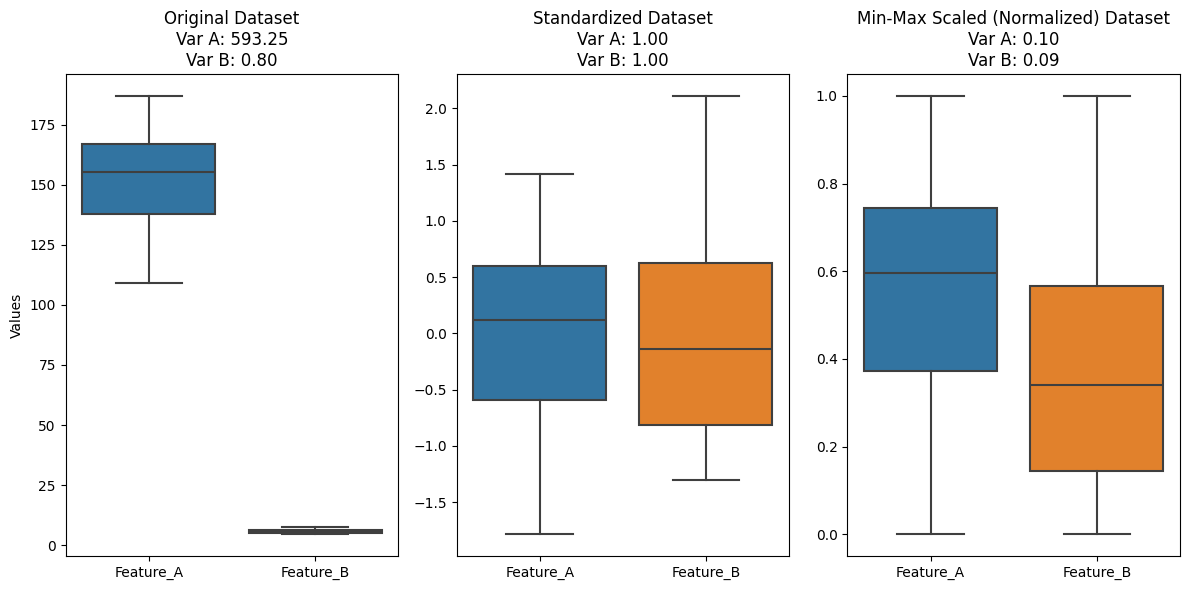
\includegraphics[width=\columnwidth]{Figures/Graphs/variance_normalization_stardization.png}
    \caption{How standardization and normalization impacts variance in datasets of different scale}
    \label{varianceImpact}
\end{figure}


\subsection{Monotonic features} \label{Monotonic-features}
Another issue is monotonically increasing features. In this dataset, these variables tend to be some form of counter. Simply throwing them in with the regular variables would add a lot of noise, as the algorithms would not know to treat them differently.
They would have to be treated differently to not be noise because they are constantly growing. In the case for counters for example, that number might mostly just reflect how long the system has been running, or some other measurement of time.
The dataset could then contain values that are consistently very low in the parts collected earlier, and consistently very high in the parts collected later in the same data collection workload.
Most machine learning algorithms would only see the change in value, and try to associate the static changes with some part of the data. This would dilute the actual information in the dataset and confuse the algorithm. \\

Here is a concrete example of the problem from the data: In one of the stress testing / collection runs, it ran for 12 minutes as usual while stress testing the "carts" endpoint.
The collected data contains several monotonically increasing variables, including a variable called "go-memstats-mallocs-total".
This Prometheus metric is from Google's Go instrumentation package, and shows how many heap objects are allocated.
It works as a counter, meaning it monotonically increases. Its value was 18387739 in the first instance of collection. 12 minutes later its value was 19284815.
An unprepared machine learning algorithm will see meaningful change in this number. Some algorithms will also just see that it has a pretty high value, and assign importance to it.
In reality, however, the correlation between system load and heap allocation is not well documented and understood in this system. More likely than not, it is as much a measure of time passing as it is a measure of system load. \\

Monotonically increasing variables can still be very useful in machine learning if treated properly.
In many cases, these variables measure something that only increases because of some factor that is relevant to the analysis at hand.
For these variables, it is often sufficient to measure the change in the value.
This change from static value to a measure of difference is a generally strong preprocessing tool, as it often can provide more meaning to algorithms \ref*{Differencing}.
However, using monotonic variables requires both good domain knowledge and good knowledge of how to transform the vairables into a format that can provide value for training.
Some monotonic features do not provide good information even when differenced, and that differencing can make them more noisy. As is demonstrated in \ref*{Differencing}, the resulting data will often seem significant and valuable.
If this is still not good data, then this will confuse the machine learning algorithm. \\
An alternative way for it to become noisy is if it is constant. In that case, differencing will turn it into a zero variance feature. As discussed earlier, this is usually noisy.
Therefore, when performing differencing and potentially mean subtraction, one should calculate variance after, and remove zero variance results.


\begin{lstlisting}[language=Python]
    
def select_by_variance(df:pd.DataFrame, amount:int):
    """
    Calculates variances, and returns the highest variance features
    Params:
    df: dataframe with time series data
    amout: the amount of features to extract
    """
    variances:pd.Series = calculate_variance(df)
    selection = variances.iloc[0:amount]
    return selection.index
best_features = select_by_variance(trimmed_df, 5)
X = scaled[best_features]
\end{lstlisting}

\begin{figure}[ht]
    \centering
    \includegraphics[width=\columnwidth]{Figures/Monotonic_differencing.pdf}
    \caption{How differencing places emphasis on changes in increment}
    \label{Differencing}
\end{figure}

\begin{figure}[ht]
    \centering
    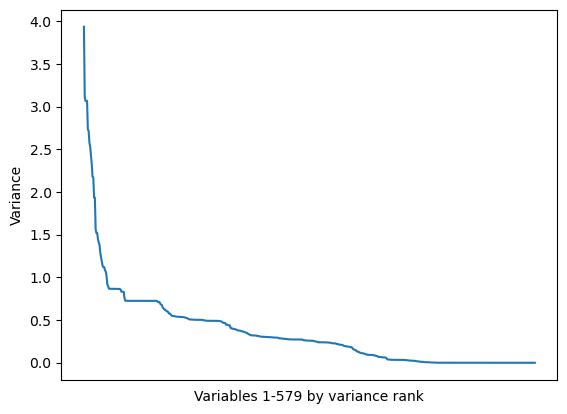
\includegraphics[width=\columnwidth]{Figures/Graphs/Total_variance}
    \caption{Scaled variance of all the variables}
    \label{variance}
\end{figure}

\subsection*{Irrelevant features}
Complex microservice systems are inherently very noisy.
Even after removing low variance features, performing imputation of missing values, differencing monotonic featues and performing dimensionality reduction, noisy features will remain.
The best tool for dealing with irrelevant features is domain knowledge, and intimate understanding of the data. This cannot always be expected when dealing with complex software. In the quite minimal example that is the dataset generated for this thesis, there are still 32 variables with 23674 datapoints for each of them.
Beyond knowledge and mastery of the specific dataset, the best idea is to hope the data is mainly relevant, and irrelevant features constitute little enough noise that it gets filtered out.
In theory, if the dataset contains features with solid correlations to the ground truth, they will override the noise from irrelevant features.

\subsection*{Non-ubiquitous features}
\label{Non-ubiquitous}
There are cases where not all the features in a dataset appear in every instance.
This will cause issues for several types of algorithms one might want to run on the data, like regression tasks, neural nets or kNN algorithms.
There are several ways of dealing with this issue.
The simplest of all is to remove all non-ubiquitous features altogether.
This requires little processing and no guessing.
It is only recommended on datasets with an abundance of features that will likely retain large amounts of information even after several features are removed.
If removing features is ill advised, or the features are only missing from a small percantage of the total amount of instances, it is possible to perform imputation of the missing features instead.
Mean or median imputation on numerical data or mode imputation on categorical data will be able to fill in missing features at the cost of some uncertainty.
This generated uncertainty can be mitigated by performing dimensionality reduction on the imputed data.
The idea is that by creating new, condensed features out of the old ones, relevant information will be brought forward and less relevant information will be obscured.
Imputed features typically carry little meaningful information, since they by design try not to say too much about the data.
In this project, Principal Component Analysis (PCA) is used to perform dimensionality reduction.\\

There are several methods of dimensionality reduction.
PCA is one of the simplest and least computationally expensive ones, as well as very common and well understood algorithm.
The drawback of PCA is mainly that it is a linear transformation:
It will always optimize for linear vector representations of the higher-dimension input data, because it uses computed eigenvalues to optimize an eigenvector to represent information in the data.
This can be a drawback if one is working with data whose information can not easily be represented by a linear vector.
This project still uses PCA because the data is theroretically linear in nature, being a standardized representation of the linear flow of time in a mostly static system.
A future improvement to the project would be to compare various means of dimensionality reduction, but it was given a low priority in this project and not included in the scope.

\begin{figure}[ht]
    \centering
    \includegraphics[width=\columnwidth]{Figures/Graphs/pca-linear.jpg}
    \caption{Demonstrating how the linearity of PCA makes it bad at approximating non-linear data. Here compared to isomap, a non-linear dimensionality reduction algorithm. Credit: https://stats.stackexchange.com/a/124545}
    \label{PCA-linearity}
\end{figure}

